\documentclass{article}

\usepackage{fancyhdr}
\usepackage{extramarks}
\usepackage{amsmath}
\usepackage{amsthm}
\usepackage{amsfonts}
\usepackage{tikz}
\usepackage[plain]{algorithm}
\usepackage{algpseudocode}
\usepackage{graphicx}
\usepackage{pgfplots}
\usepackage{subcaption}
\pgfplotsset{compat=1.18}

\usetikzlibrary{automata,positioning}

%
% Basic Document Settings
%

\topmargin=-0.45in
\evensidemargin=0in
\oddsidemargin=0in
\textwidth=6.5in
\textheight=9.0in
\headsep=0.25in

\linespread{1.1}

\pagestyle{fancy}
\lhead{Yousef Alaa Awad}
\chead{\hmwkClass\: \hmwkTitle}
\rhead{\firstxmark}
\lfoot{\lastxmark}
\cfoot{\thepage}

\renewcommand\headrulewidth{0.4pt}
\renewcommand\footrulewidth{0.4pt}

\setlength\parindent{0pt}

%
% Create Problem Sections
%

\setcounter{secnumdepth}{0}
\newcounter{partCounter}
\newcounter{homeworkProblemCounter}
\setcounter{homeworkProblemCounter}{1}

\newcommand{\hmwkTitle}{Homework\ \#3}
\newcommand{\hmwkDueDate}{March 2, 2026}
\newcommand{\hmwkClass}{Electronics 1}

%
% Title Page
%

\title{
    \vspace{2in}
    \textmd{\textbf{\hmwkClass:\ \hmwkTitle}}\\
    \normalsize\vspace{0.1in}
    \vspace{3in}
}

\author{Yousef Alaa Awad}

% \begin{figure}[!ht]
%   \centering
%   
\includegraphics[width=0.5\textwidth]{p1_42.png}
%   \caption{P1.42 from the textbook}
% \end{figure}

% Problems start here
\begin{document}

\maketitle
\pagebreak

\section{5.17}
For all the transistors in Figure P5.17, $\beta = 75$. The results of some measurements are indicated on the figures. Find the values of the other labeled currents, voltages, and/or resistor values.

\subsection{A)}
\begin{figure}[!ht]
  \centering
  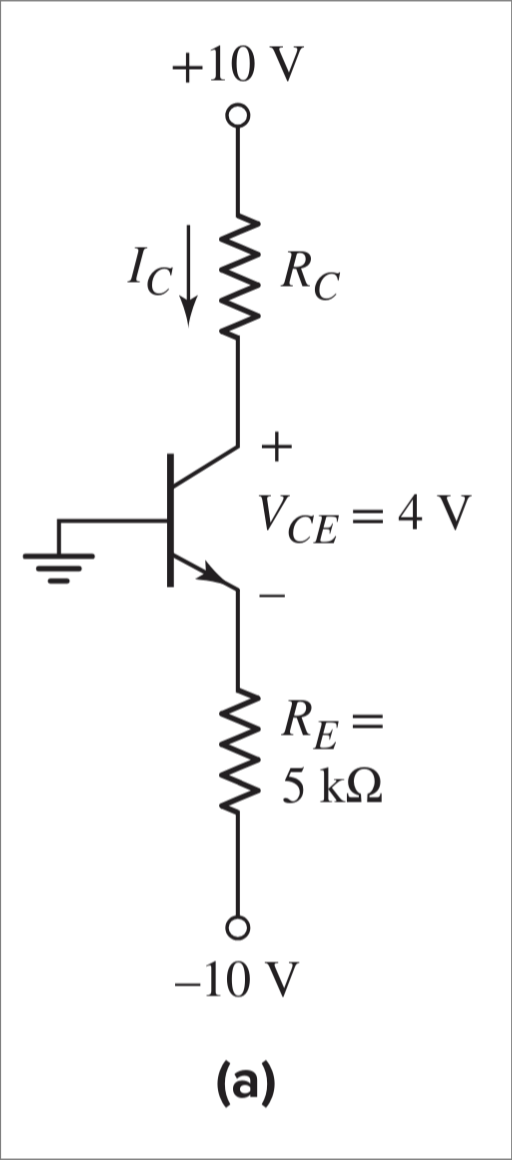
\includegraphics[width=0.2\textwidth]{517a.png}
  \caption{5.17a from the textbook}
\end{figure}
First we always assume that $V_{BE} = 0.7V$. Therefore, given we can now find out that $V_C = V_{CE} + V_E = 4 - 0.7 = 3.3$ (aka getting rid of the E portion of CE). Now, given that $I_C$ is the following:
$$ I_C = \beta*I_B \rightarrow I_B = \frac{I_C}{\beta} $$
and when plugged into the given magic equation of $I_E$:
$$ I_E = (\beta + 1)*I_B = \beta*I_B + I_B = I_C + \frac{I_C}{\beta} $$
Now, we can calculate that $I_E$ via Ohm's Law...
$$ I_E = \frac{-0.7 - (-10)}{5,000} = 1.86mA $$
And now, via our calculated $I_E$ above, we can find $I_C$:
$$ I_E = I_C + \frac{I_C}{\beta} \rightarrow 0.00186 = I_C \frac{I_C}{75} \rightarrow 0.1395 = 76*I_C \rightarrow I_C = 1.8355mA $$
Now, we can then literally do Ohm's law to find the $R_C$:
$$ I_C = \frac{10 - (4 - 0.7)}{R_C} \rightarrow \frac{0.0018355}{10 - (4 - 0.7)} = \frac{1}{R_C} \rightarrow R_C = 3650\Omega = 3.65k\Omega $$

\pagebreak
\subsection{B)}
\begin{figure}[!ht]
  \centering
  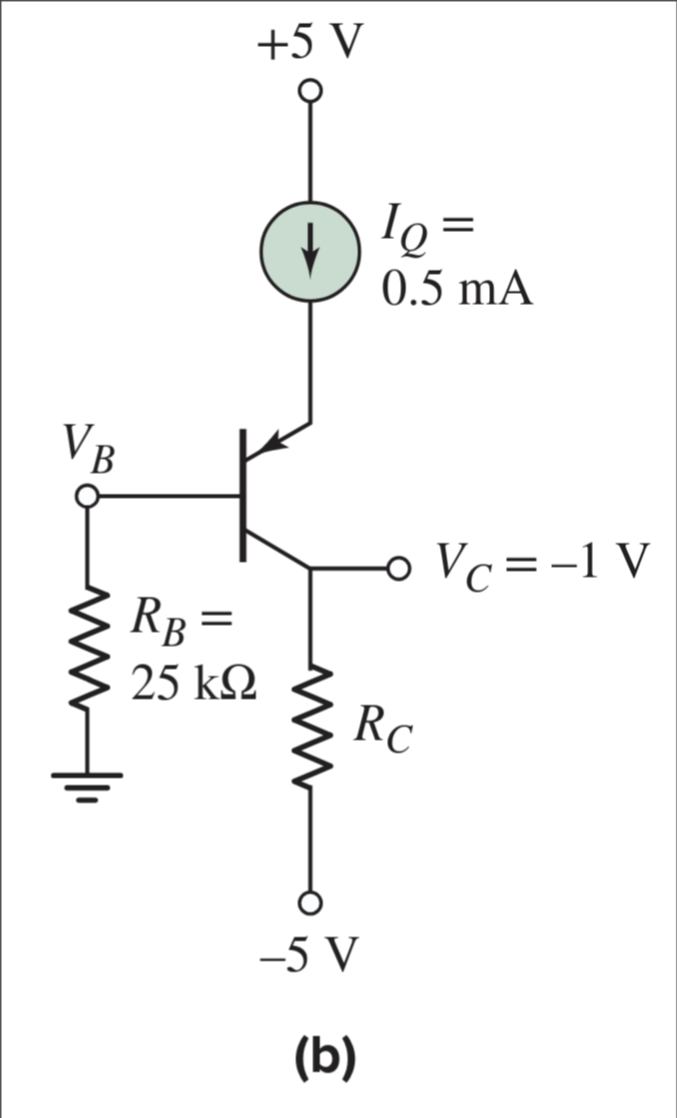
\includegraphics[width=0.2\textwidth]{517b.png}
  \caption{5.17b from the textbook}
\end{figure}
Now, we know that..
$$V_{R_C} = V_C - V_{end} = -1 - (-5) = 4V$$
But, we need to find $I_C$ so that we can use Ohm's Law. And to find $I_C$ we need to find $I_B$ and do the following, assuming that $I_Q = I_E$:
$$ I_E = (\beta + 1)*I_B \rightarrow I_B = \frac{I_E}{\beta+1} = \frac{0.5*10^{-3}}{75+1} = 6.5789*10^{-6} \rightarrow I_B = 6.5789\mu A $$
Now that we have $I_B$, we can calculate $I_C$ via...
$$ I_C = \beta*I_B = 75*6.5789*10^{-6} = 4.934175*10^{-4} = 0.4934175mA $$
And now, FINALLY, we can use Ohm's Law to find $R_C$:
$$ R_C = \frac{4}{0.434175*10^{-4}} = 8106.7\Omega $$
But, we must calculate $V_B$ via Ohm's Law as well...
$$ V_B = I_B*R_B = 6.56789*10^{-6}*25*10^{3} = 0.1644 V $$

\pagebreak
\subsection{C)}
\begin{figure}[!ht]
  \centering
  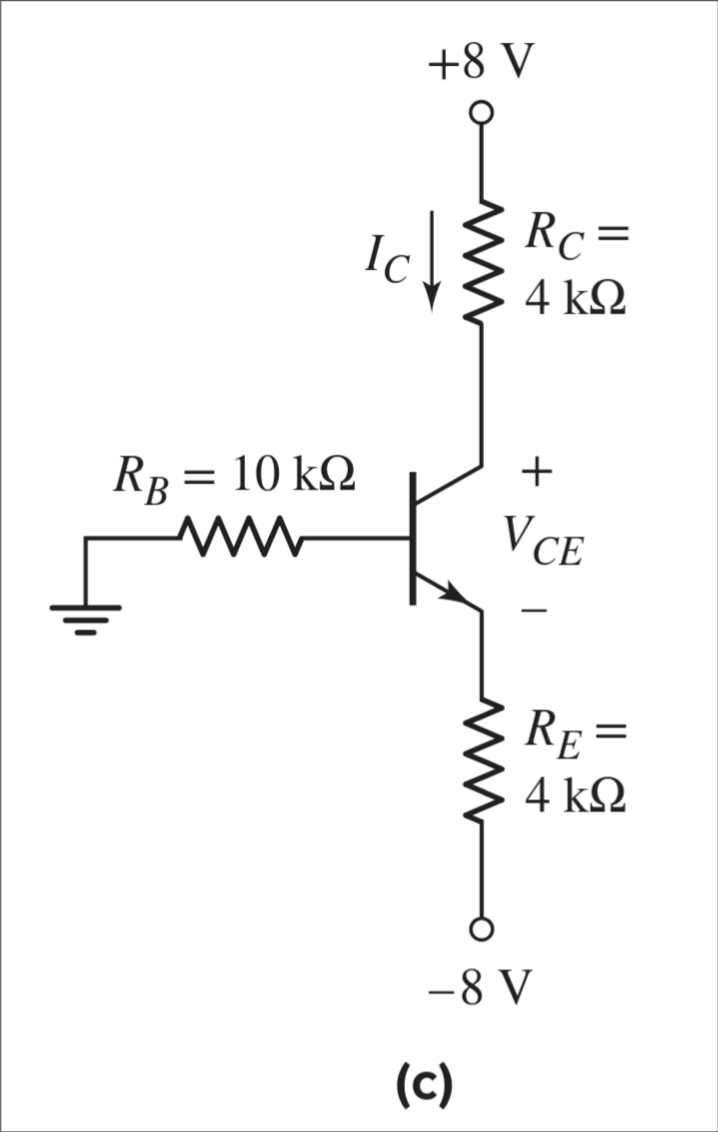
\includegraphics[width=0.2\textwidth]{517c.png}
  \caption{5.17c from the textbook}
\end{figure}
Now, we always know that $V_{BE} = 0.7V$, and that we only know resistances and the output and input voltage, therefore we must do a KVL from base's ground to the emitter's -8V to find $I_B$:
$$ R_B*I_B + V_B + R_E*I_E - 8 = 0 \rightarrow 10*10^{3}*I_B + 0.7 + 4*10^{3}*I_E - 8 = 0 $$
And when you substitute $I_E = (\beta + 1)*I_B = 76*I_B$ you get the following simplification:
$$ 10*10^{3}*I_B + 0.7 + 4*10^{3}*I_E - 8 = 0 \rightarrow 10*10^{3}*I_B + 4*10^{3}*76*I_B = 7.3 \rightarrow $$
$$ I_B = 23.23\mu A $$
Now, after calculating $I_B$, we can calculate $I_C$ via some magic equation given in class:
$$ I_C = \beta*I_B = 75*23.23*10^{-6} = 1.744mA $$
Now, we have to find $V_{CE}$, and to find that we need to first get $V_C$ via Ohm's Law:
$$ V_C + 8 = I_C*R_C = 1.744*10^{-3}*4*10^{3} \rightarrow V_C = 1.024V $$
Now we need $V_E$, but to get that we need $I_E$ and so we do the following:
$$ I_E = (\beta + 1)*I_B = 76*23.23*10^{-6} = 1.7632 * 10^{-3} = 1.7632mA $$
Now, via Ohm's Law we calculate that:
$$ V_E = I_E*R_E = 1.7632*10^{-3}*4*10^{3} \rightarrow 7.0528 - 8 = -0.9472V $$
And now we can find $V_{CE}$
$$ V_{CE} = V_C - V_E = 1.024 - (-0.9472) = 1.9712V $$

\pagebreak
\subsection{D)}
\begin{figure}[!ht]
  \centering
  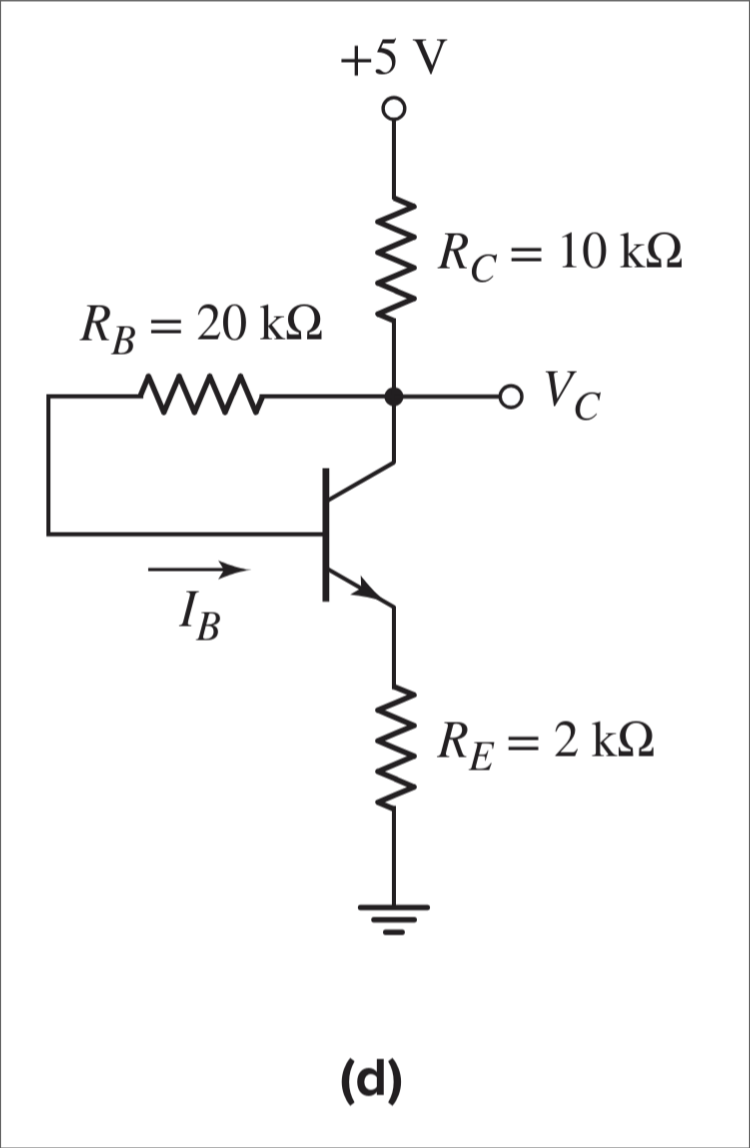
\includegraphics[width=0.2\textwidth]{517d.png}
  \caption{5.17d from the textbook}
\end{figure}
Now, we always assumed that $V_{BE} = 0.7V$ and therefore we do a KVL to find $I_B$:
$$ 5 - 10*10^{3}*I_C - 20*10^{3}*I_B - 0.7 - 2*10^{3}*I_E = 0 \rightarrow 5 - 10*10^{3}*I_B - 20*10^{3}*I_B - 0.7 - 2*10^{3}*(\beta + 1)*I_B = 0 $$
$$ \rightarrow I_B = 4.664\mu A $$
Now, we also then can calculate $I_C$:
$$ I_C = \beta*I_B = 75*4.664*10^{-6} = 0.350mA $$
And now we can use Ohm's Law to find $V_C$:
$$ 5 - V_C = I_C*R_C \rightarrow 5 - V_C = 0.350*10^{-3}*10*10^{3} \rightarrow V_C = 1.502V $$

\pagebreak
\section{5.23}
In the circuits shown in Figure P5.23, the values of measured parameters are shown. Determine $\beta$, $\alpha$, and the other labeled currents and voltages. Sketch the dc load line and plot the Q-point.

\subsection{A)}
\begin{figure}[!ht]
  \centering
  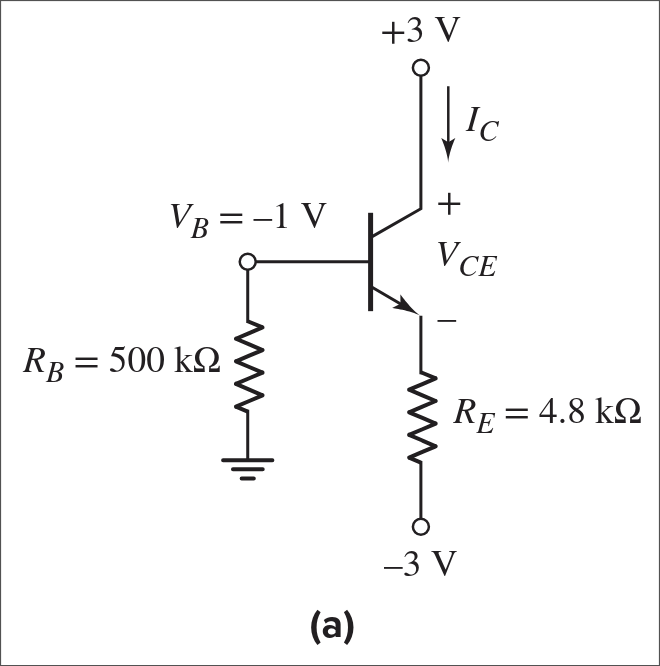
\includegraphics[width=0.4\textwidth]{523a.png}
  \caption{5.23a from the textbook}
\end{figure}
First we must try and find the $\beta$ value. And to do that, we must find 2 respective currents that can therefore be transferred to each other.
$$ I_B = \frac{0 - (-1)}{500*10^{3}} = 2*10^{-6} = 2\mu A $$
$$ I_E = \frac{-1.7 - (-3)}{4.8*10^{3}} = 0.271*10^{-3} = 0.271mA $$
And now, given $I_E = (\beta + 1)*I_B$, we can find $\beta$:
$$ I_E = (\beta + 1)*I_B \rightarrow 0.271*10^{-3} = (\beta + 1)*2*10^{-6} \rightarrow \beta = 134.317 $$
And now that we have $\beta$, we can calculate $\alpha$:
$$ \alpha = \frac{\beta}{\beta + 1} = \frac{134.317}{134.317 + 1} \rightarrow \alpha = 0.993 $$
Now, the only this left is to find $I_C$ and $V_{CE}$. First I shall find $I_C$:
$$ I_C = \beta*I_B = 134.317*2*10^{-6} = 0.269mA $$
And now, $V_CE$. For this, the figure shows that $V_C = 3V$, therefore $V_{CE}$ is the following:
$$ V_{CE} = 3 - V_E = 3 -( -1 -0.7) = 3 + 1.7 = 4.7V $$

\subsubsection{Graph}
\begin{center}
\begin{tikzpicture}[scale=1]
    % Draw the X and Y axes
    \draw[->, thick] (-0.5,0) -- (5,0) node[right] {$V_{CE}$ (V)};
    \draw[->, thick] (0,-0.5) -- (0,4) node[above] {$I_C$ (A)};
    
    % Draw the load line
    \draw[thick] (0,3) -- (4,0);
    
    % Define the Q-Point coordinates
    \coordinate (Q) at (2,1.5);
    
    % Draw the Q-Point dot and label it
    \filldraw (Q) circle (1.5pt) node[above right] {Q-Point};
    
    % Draw dashed lines connecting the Q-Point to the axes
    \draw[dashed] (Q) -- (2,0) node[below] {$4.7\text{ V}$};
    \draw[dashed] (Q) -- (0,1.5) node[left] {$0.269\text{ mA}$};
    
\end{tikzpicture}
\end{center}

\subsection{B)}
\begin{figure}[!ht]
  \centering
  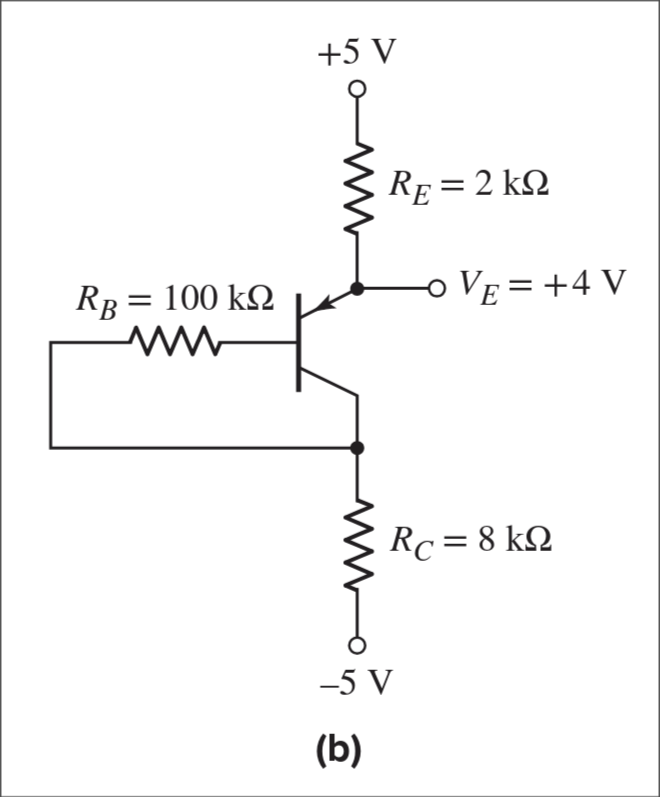
\includegraphics[width=0.4\textwidth]{523b.png}
  \caption{5.23b from the textbook}
\end{figure}
First we can find $I_E$:
$$ I_E = \frac{5-4}{2*10^3} = 0.5*10^3 = 0.5mA $$
After this, we can find $V_B$ since $V_{BE} = 0.7V$:
$$ V_{BE} = V_B - V_E \rightarrow -0.7 = V_B - 4 \rightarrow V_B = 3.3V $$
After this, we do a KCL to find $I_C$, and therefore the rest of the stuff we need.
$$ I_E = I_C + I_B $$
And since the emitter is facing the transistor (it's a PNP), it means that all current is heading towards the collector. Therefore...
$$ I_C = I_E + I_B $$
Therefore...
$$ I_{R_C} = I_E $$
Therefore, we can find $V_{R_C}$ via Ohm's Law:
$$ V_{R_C} = -5 + 0.5*10^{-3}*8*10^3 \rightarrow V_{R_C} = -1V $$
NOW, WE CAN FIND THE CURRENT IN THE BASE!!!!!! I LOVE BASE, AND HATE TREBLE BTW:
$$ V_{R_B} = V_B - V_{R_C} = 3.3 - (-1) = 4.3V $$
NOW, OHM'S LAW:
$$ I_B = \frac{4.3}{100*10^3} = 0.43*10^{-6} = 0.43\mu A $$
NOW, BETA:
$$ I_E = (\beta + 1)*I_B \rightarrow 0.5*10^{-3} = (\beta + 1)*0.43*10^{-6} $$
$$ \beta = 10.6279 $$
And $\alpha$ is...
$$ \alpha = \frac{\beta}{\beta + 1} = 0.914 $$

\subsubsection{Graph}
\begin{center}
\begin{tikzpicture}[scale=1]
    % Draw the X and Y axes
    \draw[->, thick] (-0.5,0) -- (5,0) node[right] {$V_{CE}$ (V)};
    \draw[->, thick] (0,-0.5) -- (0,4) node[above] {$I_C$ (A)};
    
    % Draw the load line
    \draw[thick] (0,3) -- (4,0);
    
    % Define the Q-Point coordinates
    \coordinate (Q) at (2,1.5);
    
    % Draw the Q-Point dot and label it
    \filldraw (Q) circle (1.5pt) node[above right] {Q-Point};
    
    % Draw dashed lines connecting the Q-Point to the axes
    \draw[dashed] (Q) -- (2,0) node[below] {$5\text{ V}$};
    \draw[dashed] (Q) -- (0,1.5) node[left] {$0.457\text{ mA}$};
    
\end{tikzpicture}
\end{center}

\pagebreak
\section{5.29}
For the circuit shown in Figure P5.29, if $\beta = 200$ for each transistor, determine: (a) $I_{E1}$, (b) $I_{E2}$, (c) $V_{C1}$, and (d) $V_{C2}$.
\begin{figure}[!ht]
  \centering
  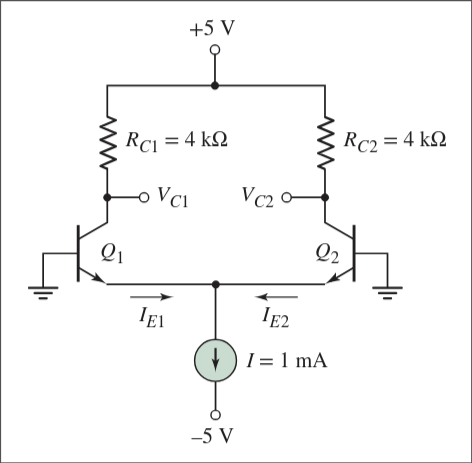
\includegraphics[width=0.4\textwidth]{529.png}
  \caption{5.29 from the textbook}
\end{figure}

\subsection{A)}
To calculate $I_{E1}$, we must first realize that $I_{E1}$ and $I_{E2}$ are equal due to how the circuit is symmetrical. Due to this, we can know the following:
$$ I_{E1} + I_{E2} = 1mA \rightarrow I_{E1} = I_{E2} = 0.5mA $$

\subsection{B)}
Since we established $I_{E1}$ and $I_{E2}$ are equal, then we have already calculated $I_{E2}$...
$$ I_{E2} = I_{E1} = 0.5mA $$

\subsection{C)}
To calculate $V_{C1}$, we first must find $I_{C1}$. And to do that, we have to realize that $I_C1$ will be the same as $I_E1$ since the $V_B$ is 0V. Since that is true, we then can use Ohm's Law to find that $V_{C1}$ is...
$$ 5 - V_{C1} = 0.5*10^{-3} * 4*10^3 \rightarrow V_{C1} = 3V $$

\subsection{D)}
Since we established that both sides are symmetrical, then we have already calculated $V_{C2}$...
$$ V_{C2} = V_{C1} = 3V $$

\pagebreak
\section{5.49}
For the transistor in the circuit shown in Figure P5.49, assume $\beta = 120$. Design the circuit such that $I_{CQ} = 0.15 mA$ and $R_{TH} = 200 k\Omega$. What is the value of $V_{CEQ}$?
\begin{figure}[!ht]
  \centering
  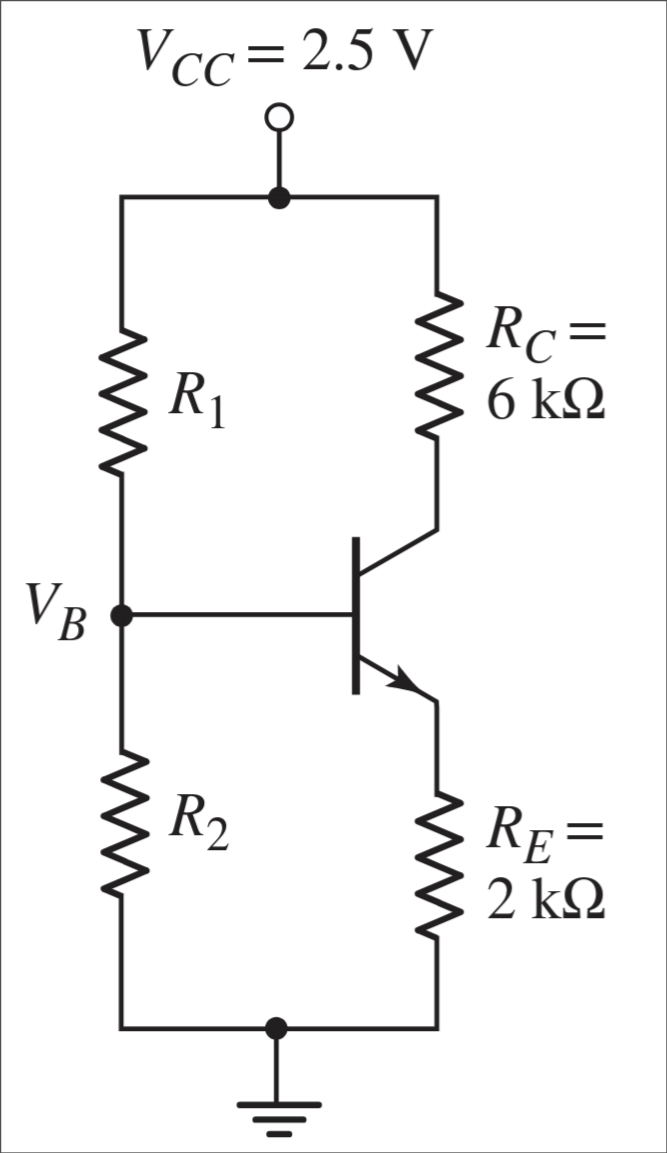
\includegraphics[width=0.3\textwidth]{549.png}
  \caption{5.49 from the textbook}
\end{figure}

First, we are given $I_{CQ}$, therefore we can find $V_C$:
$$ V_{R_C} = I_{CQ}*R_C = 0.15*10^{-3}*6*10^{3} = 0.9V $$
Therefore, $V_C$ will be...
$$ V_C = 2.5 - 0.9 = 1.6V $$
Now we can calculate $V_B$ via the given magic equations from the ether:
$$ I_B = \frac{I_C}{\beta} = \frac{0.15*10^{-3}}{120} = 1.25*10^{-6} = 1.25\mu A $$
After this we sadly cannot find $V_B$ yet, BUT we can find $I_E$.
$$ I_E = (\beta + 1)*I_B = 0.15125*10^{-3} = 0.15125mA $$
Now, we can find $V_E$, of which we know is via Ohm's Law!
$$ V_E = I_E * R_E = 0.15125*10^{-3} * 2*10^{3} = 0.3025V $$
And!!! After this, we know that $V_BE$ is ALWAYS 0.7V, therefore we simply have to add 0.7V to whatever our $V_E$ is to find $V_B$:
$$ V_B = V_E + 0.7 = 1.0025V $$
And, with this we know $V_{CEQ}$:
$$ V_{CEQ} = V_C - V_E = 1.6 - 0.3025 = 1.2975V $$
Now, we need to find $R_1$, and $R_2$. And to do that, we will assume that $V_B$ is where the the load of the thevenin circuit is. Therefore, because the load gives out a "voltage" of 1.0025V, and a current of $1.25\mu A$, we can calculate via Ohm's Law, that $V_{TH}$ to be:
$$ V_{TH} = 200*10^{3}*1.25*10^{-6} + 1.0025 = 1.2525V $$
After this, given from the magic lab.... 
$$ V_{TH} = \frac{V_{CC}*R_2}{R_1 + R_2} \rightarrow 1.2525 = \frac{2.5*R_2}{R_1 + R_2} \rightarrow 1.004008*R_1 = R_2 $$
And now, we just assume its bloody parallel (thank you lab):
$$ R_{TH} = \frac{R_1*R_2}{R_1 + R_2} \rightarrow 200*10^3 = \frac{1.004008*R1^2}{2.004008*R_1} \rightarrow $$
$$ R_1 = 399,201.6\Omega $$
$$ R_2 = 400,801.6\Omega $$


\end{document}

